\chapter{CEMicro Architecture and Technology Stack}
\label{sec:arch}

This chapter takes us through the journey of planning and designing the CEMicro service. We understand the boundaries and features of the so-called ``Configurable Elements'' of the POS application and learn the goals Capgemini has with this project. Several times initial assumptions about the final service are challenged, and new and better design decisions made. We also decide, or sometimes somewhat justify, the technology decisions for the later implementation of CEMicro.

\begin{figure}[ht]
  \centering
  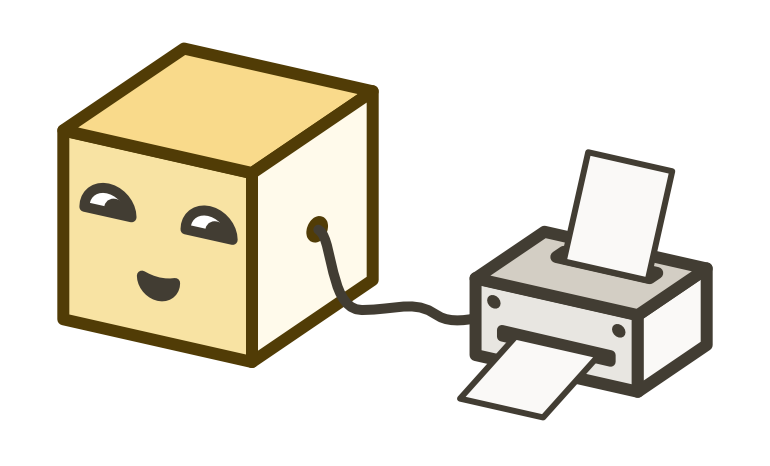
\includegraphics[width=0.4\linewidth]{assets/illustration-microservice-printer.png}
  \caption{CEMicro is responsible for the ``Configurable Elements'' of printed documents}
\end{figure}

\section{The existing appliction}

The existing application which this department of Capgemini is working on is a point of sales (POS) software. It is essentially the toolkit a salesman uses to create an offer for a potential customer. Since cars are a highly configurable product, the POS software has to support a wide variety of options. It is made even more complicated by the different types of cars, different types of brands, or sub-brands, and the fact that it is in use across several markets and languages. Each market has its very own requirements and levels of hierarchy, which the application reflects in terms of user management and access levels.

The part of the application which involved my task is the creation of the final offer as a printable PDF document. Depending on the object of the sale, the type of car, the current market, and a host of other factors, the application will decide which document template to use. It will then collect the appropriate lines of text and values from the database to assemble into a finished document, which it then generates in the PDF format. Additionally, there are several configuration pages in the admin area of the application that manages these templates and defines their contents. Figure \ref{fig:pos} shows a glimpse of the somewhat unwieldy admin interface for the part of the document creation.

There are currently nine teams of about six developers, each working on the POS application.

\begin{figure}
  \begin{subfigure}[b]{0.5\linewidth}
    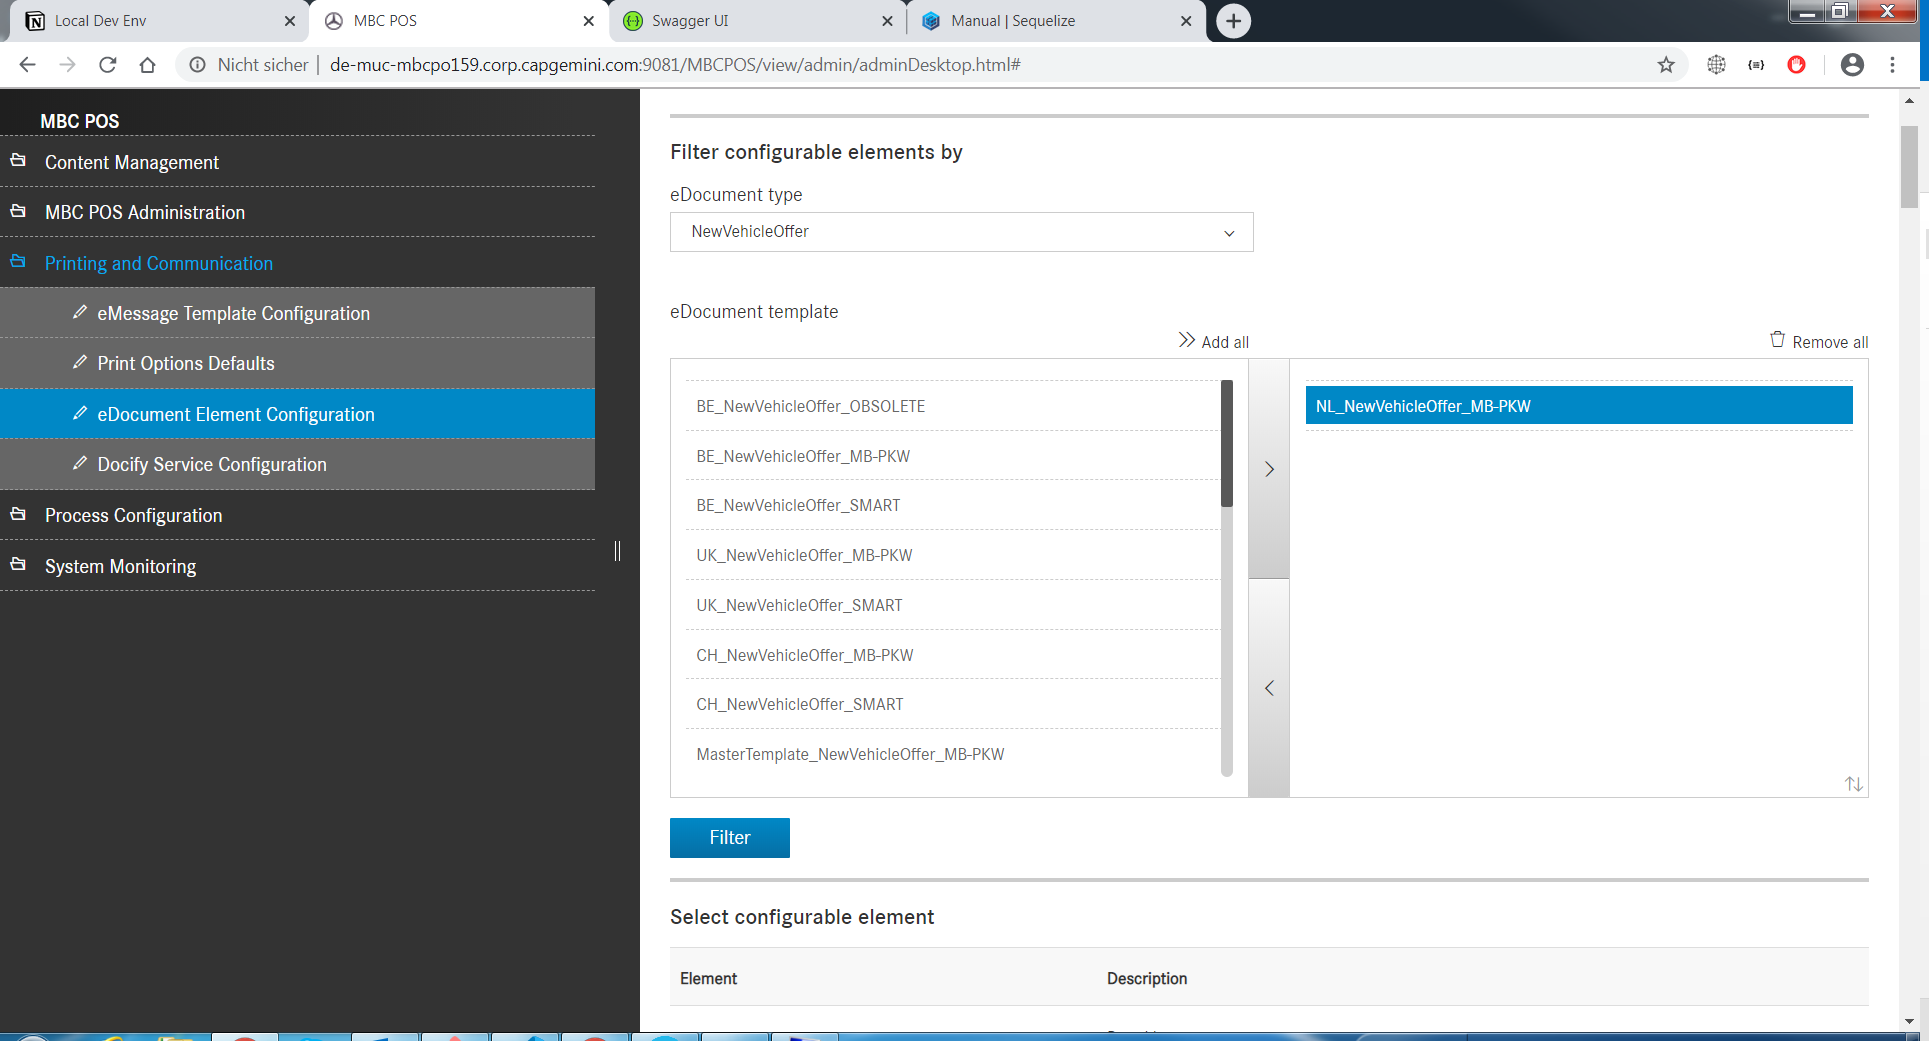
\includegraphics[width=\linewidth]{assets/pos-ce-config-1.png}
    \caption{Template selection}
    \label{fig:pos:a}
  \end{subfigure}
  \begin{subfigure}[b]{0.5\linewidth}
    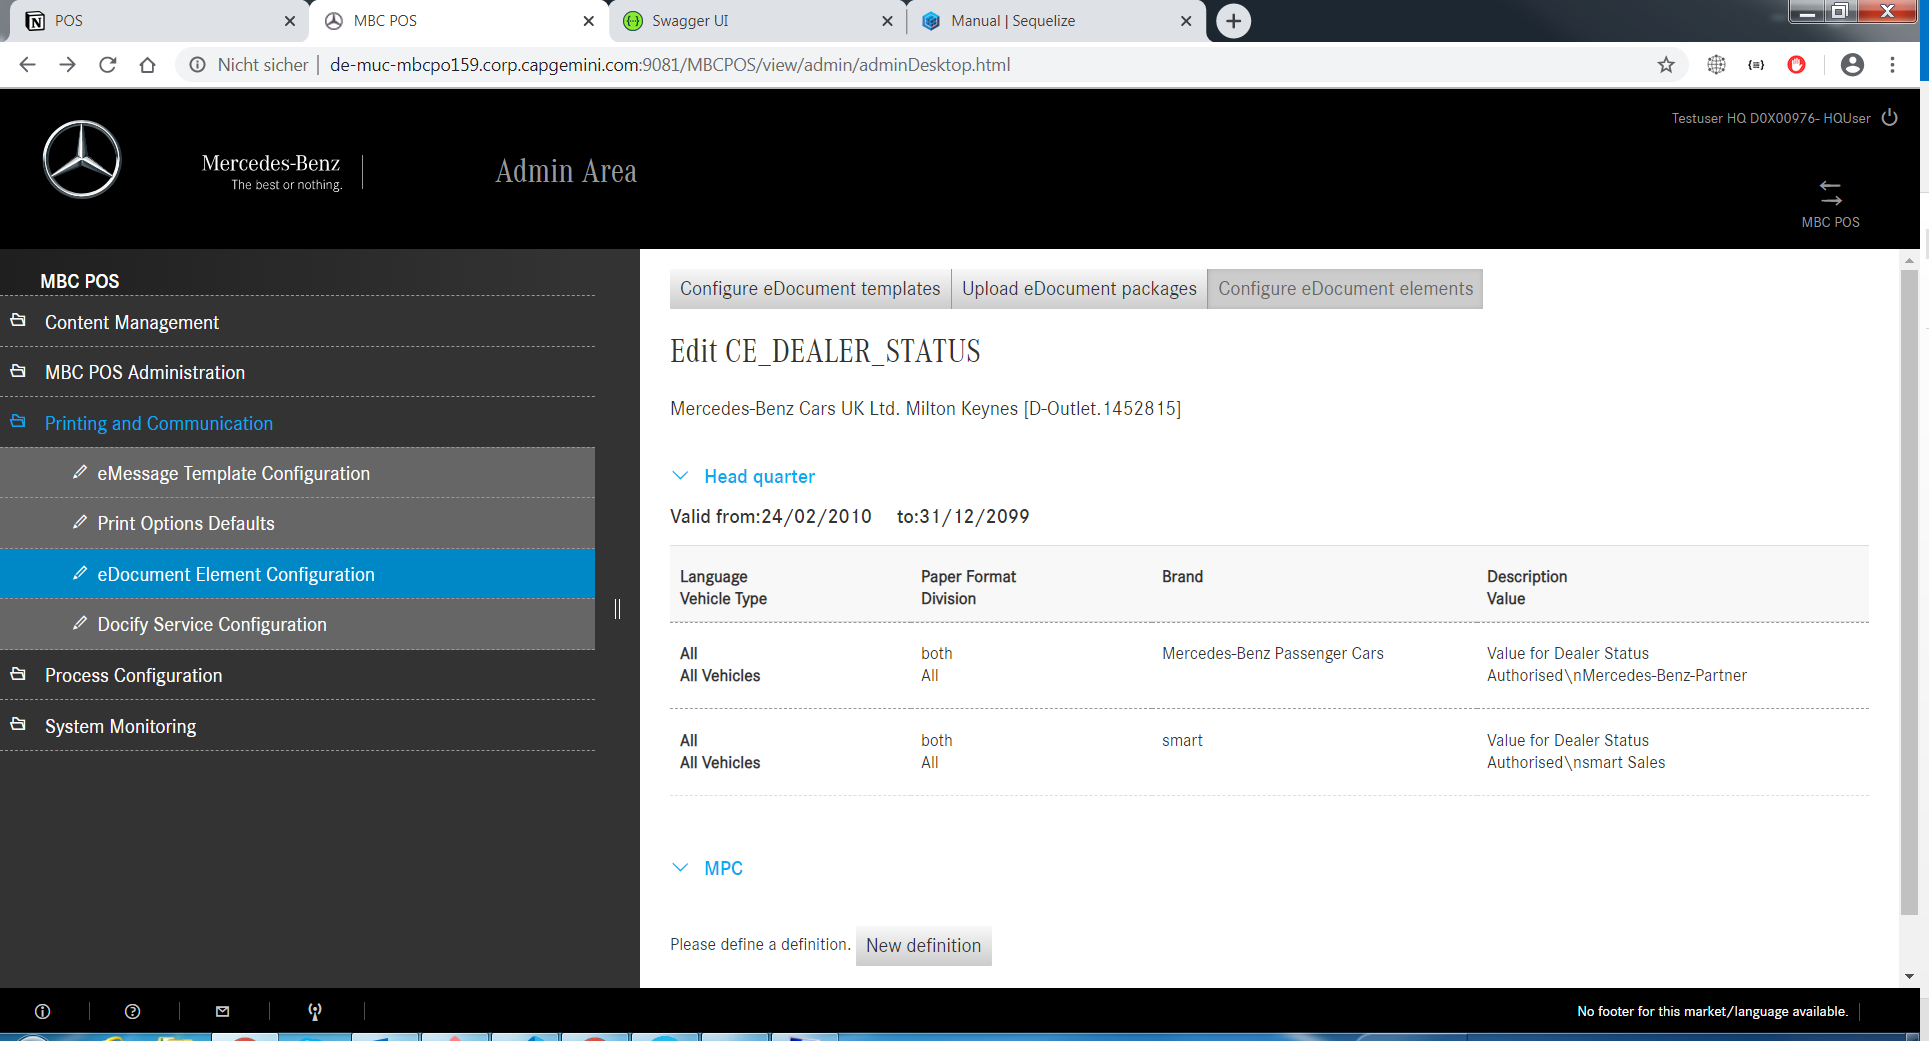
\includegraphics[width=\linewidth]{assets/pos-ce-config-3.png}
    \caption{One CE contains several children}
    \label{fig:pos:b}
  \end{subfigure}
  \caption{POS configurable element admin page}
  \label{fig:pos}
\end{figure}

The part of the application responsible for generating a printable document has been part of a past student project very similar to my task. The team of students essentially built a microservice that is responsible for managing the templates. An application programming interface (API) provides access to the service and returns the finished PDF. They called this service Docify.

Docify is a kind of textbook example for a microservice. A document printing service lends itself very nicely to be extracted into its separate application because its interface is so clearly defined. The interface for a printing service requires two properties, first, the name or identifier of the predefined template, and second, the dataset which is needed to fill the gaps of the template. That often means the biggest challenge for distributed services, defining the boundaries, and thus their interfaces are no-brainers for this use-case.

Figure \ref{fig:docify} shows the administration interface for Docify, and it is easy to see how each of the two previously mentioned API criteria has its page. On the left \ref{fig:docify:a} is the list of templates, the identifier of each template is a client-market-name tuple, and on the right \ref{fig:docify:b} is the editor for template specific templates with the HTML representation on the left and the rendered preview. The HTML code contains several placeholders which replace their respective value when printing document.

\begin{figure}
  \begin{subfigure}[b]{0.5\linewidth}
    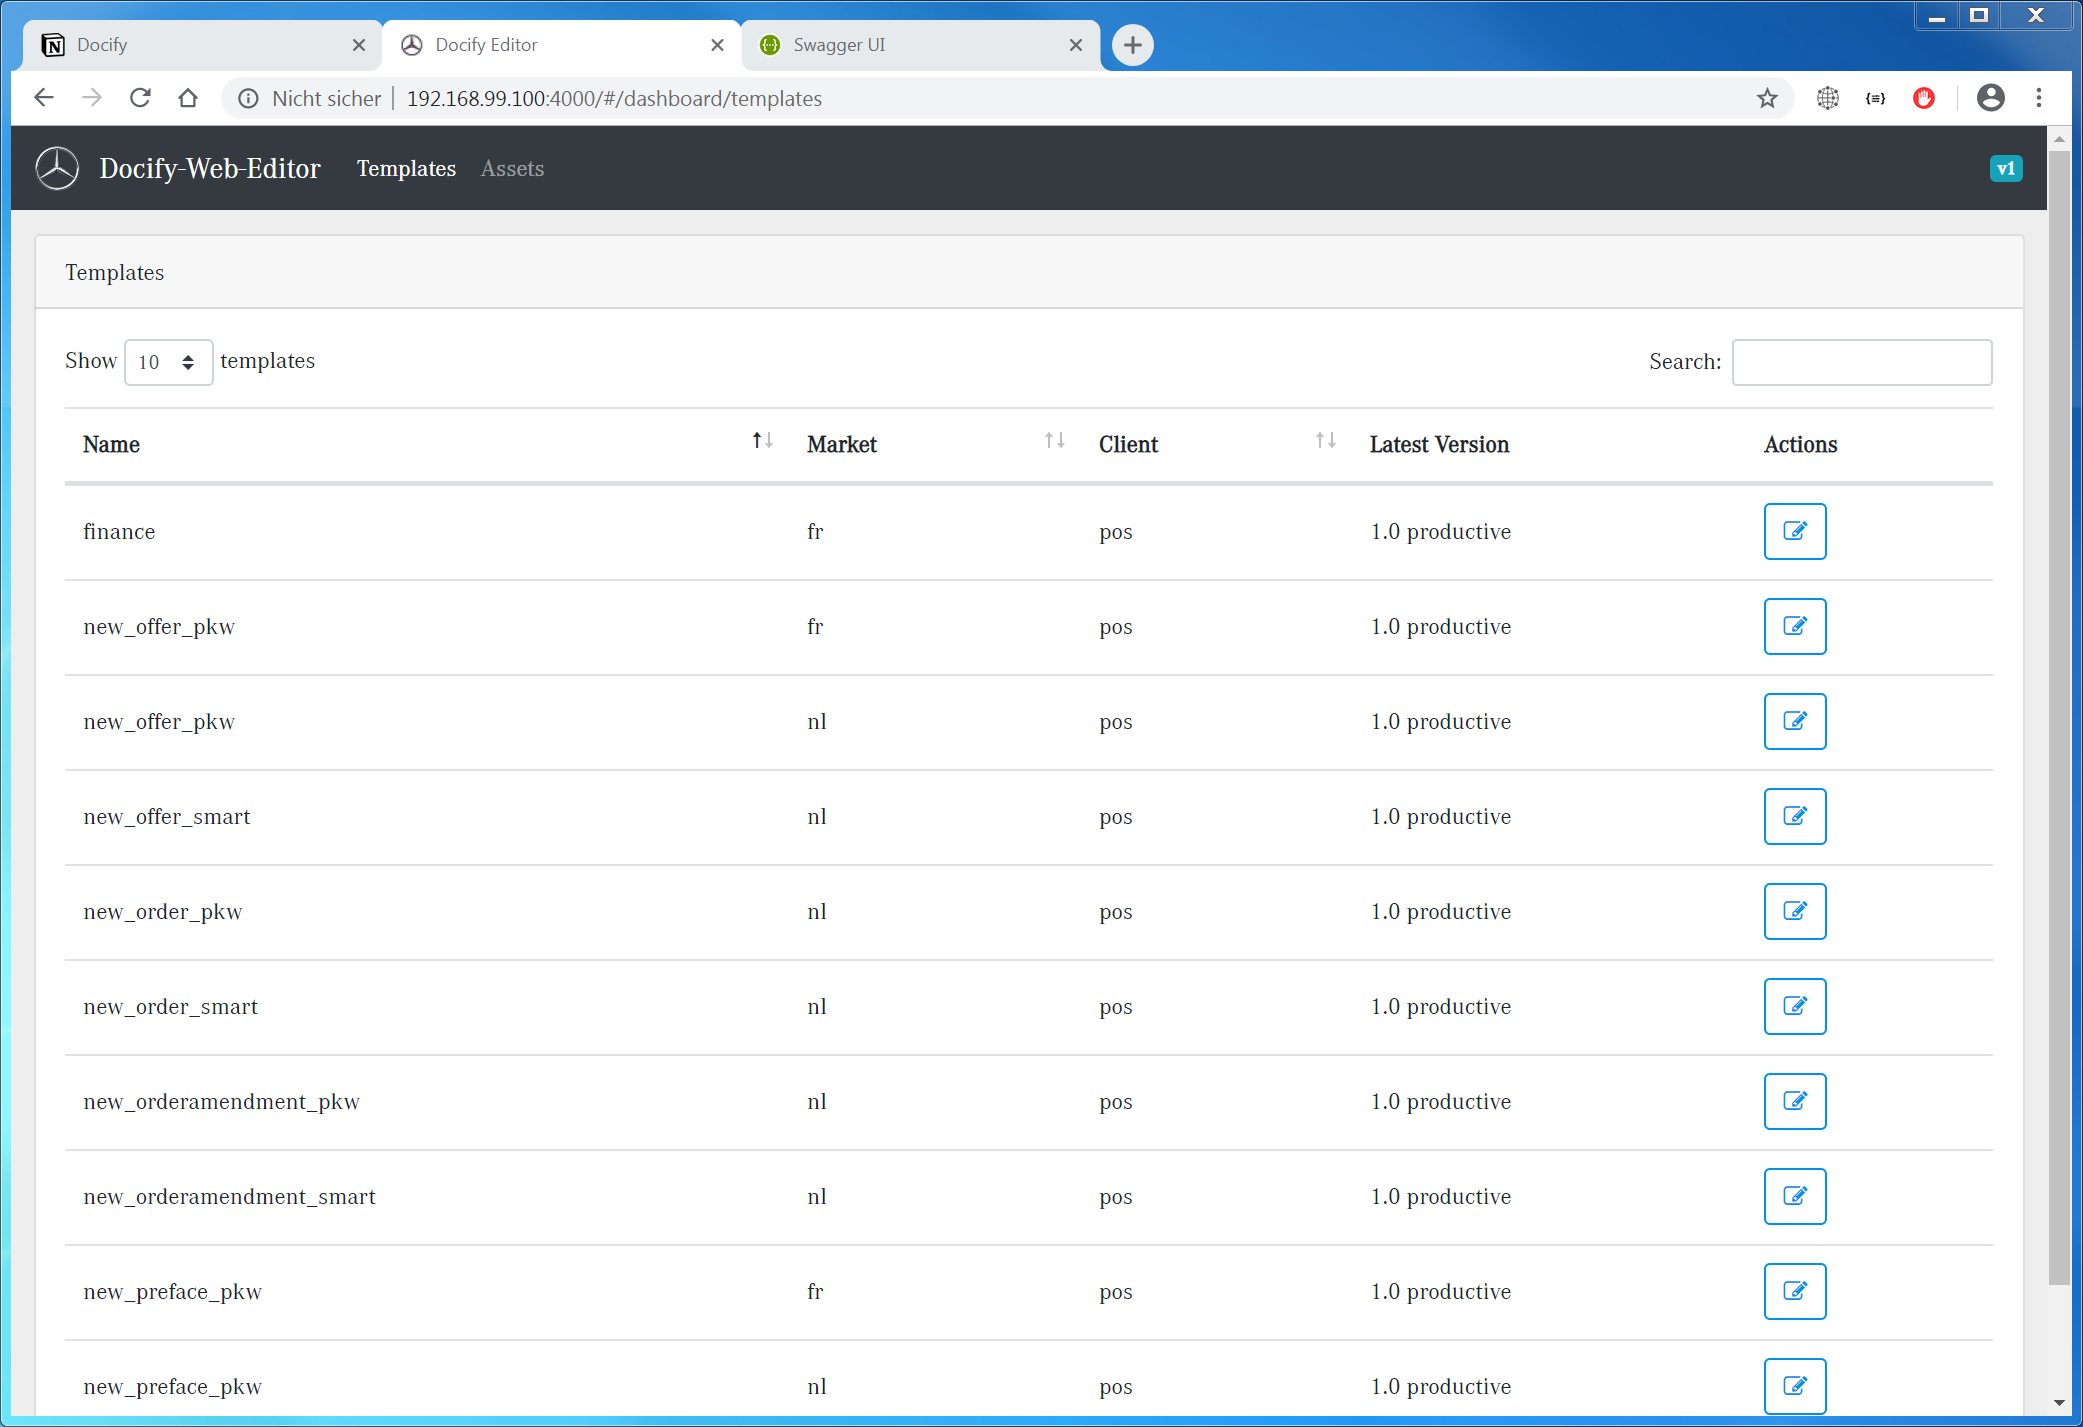
\includegraphics[width=\linewidth]{assets/docify-template-list.png}
    \caption{Template list}
    \label{fig:docify:a}
  \end{subfigure}
  \begin{subfigure}[b]{0.5\linewidth}
    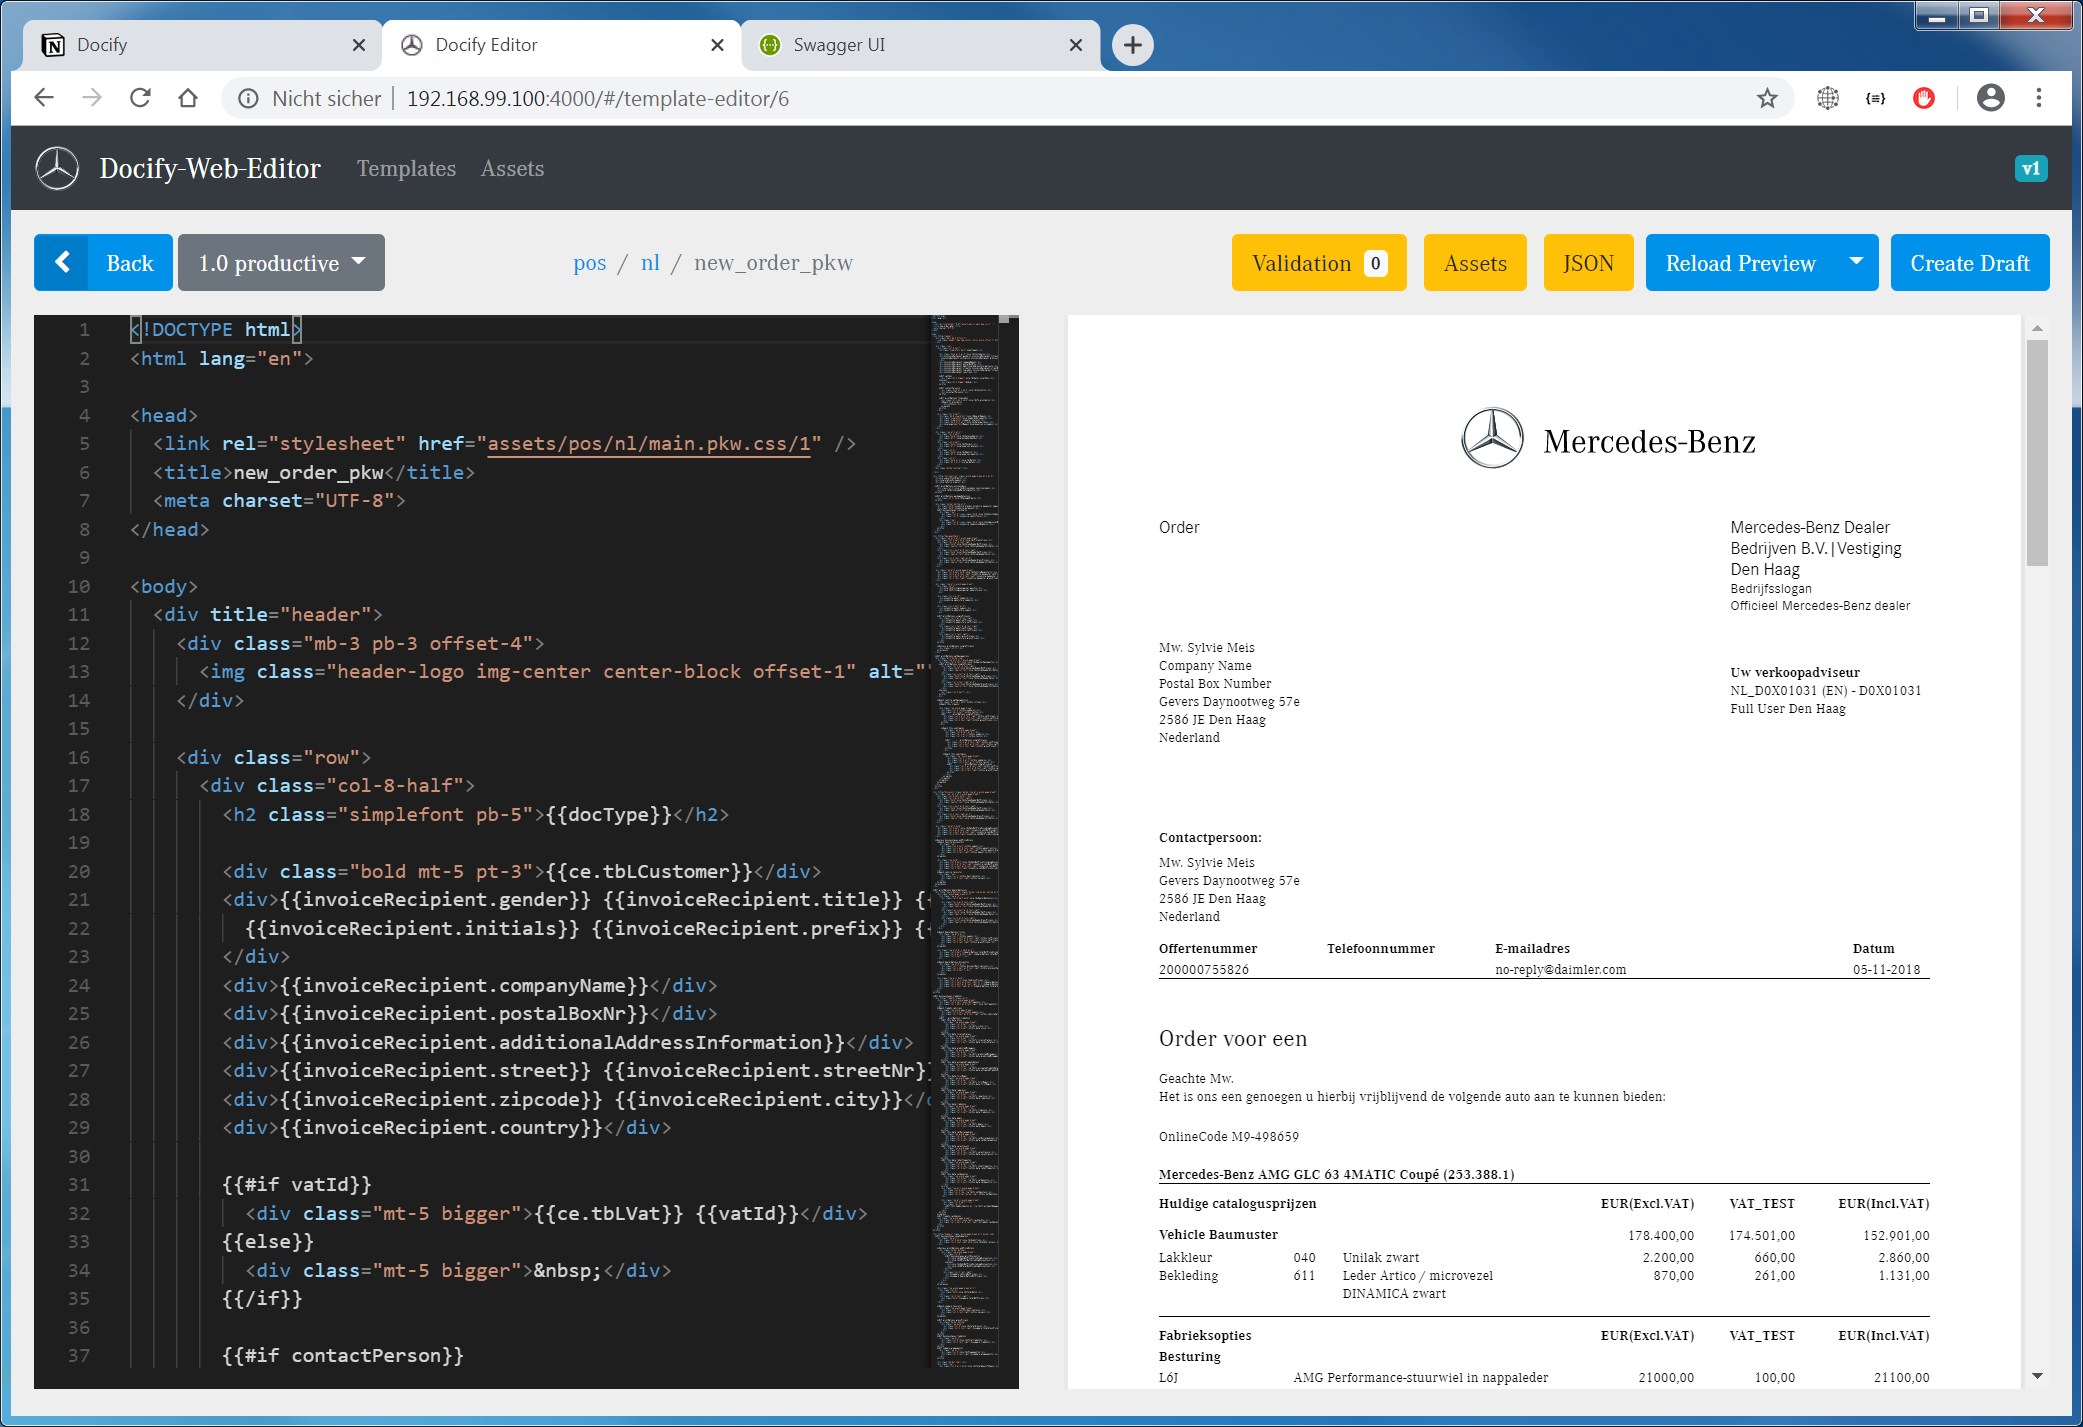
\includegraphics[width=\linewidth]{assets/docify-editor.png}
    \caption{Template editor}
    \label{fig:docify:b}
  \end{subfigure}
  \caption{Docify template editor app}
  \label{fig:docify}
\end{figure}

While the technical aspect of Docify might be simple, it is interesting to observe the non-technical challenges that a microservice is facing. Besides the question of how a microservice should be extracted and build, there is the economic question of why it is necessary to invest the time into creating such a service when it seems to be working just fine as it is. The question every project has to face is, ``Does it add business value?'' and if it doesn't, why should the business spend money on the project? This is an interesting question especially for engineers who often try to build the ideal solution for a problem, after all, that's why we became engineers in the first place, but forget that our time is valuable and to build the ideal solution, in this case, a microservice, for an already working feature may not make much sense to the business as a whole.

So why was Docify build in the first place? I haven't been involved myself, but from the proceedings with my project, I can surmise some good indicators. On the one hand, the POS application is over five years old, which in the world of software is a man with a cane and a white beard. Over the lifetime of any software, it tends to become ever more complex and both in its technical scope but also in terms of management. Thus even small changes to the codebase can take several days or even weeks until the task gets prioritized, implemented, and deployed. In the ideal situation, the database contains all the parts which users are supposed to be able to edit so that changes don't have to be handed to developers, but in the case of POS, many adjustments to the document creation could only be made by direct manipulation of the codebase which meant that a task had to be created for developers.

One example of this directly involves my task, the so-called ``Configurable Elements,'' which I will describe in more detail in the next section, are basically texts that can be edited by users. But the definition for these elements is hardcoded in the application, meaning if users want to add a new such item, they have to create a task for devs to do so, which adds considerable friction to something which should be just one click. Essentially, Docify enables users to do administrative tasks directly while saving all the development time of adding these admin interface features to the existing monolith codebase.

The other business value has to do with the fact that there is currently a particular hype around microservice architectures. The project of Docify enabled Capgemini to showcase this architectural model on a reasonably simple use-case to its client while not losing much in terms of wasted development time if the client declines its further development. And since a microservice can be built in a completely separate tech stack, it was mostly a proof of concept/demo of a flashy new architecture and some flashy new technology.

In the end, the client liked what business value Docify had to offer and was willing to invest in its development. At the time of this writing, Docify is two years old and was rolled out to two of the several markets POS is operating in. Meaning even after two years of development, the POS team is still maintaining the old implementation in spite of the new and shiny microservice, which is probably an appropriate image of how large companies tend to operate if their internal structures became sufficiently complex.


\section{Goals of the CEMicro Service}

\begin{itemize}
  \item \done{What is the microservice supposed to do}
  \item \done{High-Level Overview of Illustration}
  \item \done{The complexity of POS / CE Properties}
  \item \done{Out of scope: Access control}
\end{itemize}


As already noted in the previous segment, the idea of a microservice for document creation is pretty straightforward since the API is well defined from the get-go. The printable document handling in POS, however, has three parts. Besides template and dynamic values, which are different on a per offer basis, it defines a number of static values inside the templates, which are called ``configurable elements.'' The idea behind configurable values, or CEs in short, is, that they are the same on every printout, but can be defined according to a number of factors like the current language if the paper is branded or blank if a new or used car is sold and so on.

The next segment will go into more detail what complexity was actually hidden behind the rather primitive looking CEs but suffice to say at this point, the setting of these static values for a printable template is cumbersome and complicated by nature.

My task, therefore, was to extract the configuration of these CE values into a separate service, which can be queried by the POS system to retrieve the correct set of CE values for any given document template under a given set of conditions. For example, if the salesman using POS wants to print an offer for a new car in the Netherlands on blank paper, the POS application would then send a request to this new service saying: ``please give me all the configurable elements I need to print a new offer for this and that car in the Netherlands marked on blank paper.'' The responsibility of the service would then be to produce a list of key-value pairs that the POS application can then hand to the Docify service, or its internal printing function for that matter, to be inserted into the configurable element placeholders in the document template.

Not much guidance was given to me beyond this point from Capgemini. I was given access to the source code of both the POS application and the Docify service and could start them on personal virtual machines to understand their working. Because several teams of developers were working on POS and after seeing the size of the codebase, I quickly concluded that it would not make much sense for me to try to understand the inner workings of the existing Java code. Instead, I decided to investigate the user interface of both services, and in the case of Docify, the API to understand what features my service needs to offer and what interfaces it should expose.

I decided to call the service CEMicro, short for Configurable Element Microservice. The name is rather dull and not in the vain of more modern hipster names like Spotify or Instagram, but it serves a very functional purpose in quickly communicating what it is supposed to do to an audience that is familiar with the existing cumbersome feature of configurable elements. I felt choosing a functional name that eases the adoption of a new service was more expedient than a beautiful and fancy name.

Early in the planning of the application context, that is, with whom the new application needs to communicate about what, I assumed that CEMicro only needs to talk to the POS system since, in the end, only the POS system will request a dataset from CEMicro. But after understanding that the templates are actually not available to POS but rather maintained by Docify, it became clear to me that either CEMicro has to have its own copy of each template or it needs to request the template from Docify in order to know which configurable elements the template requires. Another option would have been for users to tell CEMicro which configurable elements exist and are part of which template, but this would have meant a double effort for users since each new CE that was defined inside a template in Docify needs to be additionally added to CEMicro, which brings us to the concept of the single source of truth.

The single source of truth \todo{[ref]} is a fundamental concept in programming that value or variable should only be defined and maintained in one place, the source of truth. As soon as they are set in multiple locations, there has to be a system to keep each other synchronized; otherwise, the application state will be inconsistent. The single source of truth principle thus becomes even more critical for a distributed service architecture. In a monolith application, and this is really the reason why monoliths are more comfortable to develop and more widely used, there is usually only one database, and the whole application has access to all the data. But in a distributed service architecture, every individual service only has its own database. In order to make this work, each service can only handle the data of its particular domain and has to request the data of other services through their public interfaces. In the case of CEMicro, the database can only contain the data of the actual configurable elements and not the data of the templates, or the user table for that matter. If copies of a dataset existed in the databases of multiple services, there would need to be a mechanism to keep all these copies in sync. This can be done through a publish-subscriber pattern \todo{[ref]}, but if the availability of the network can not be guaranteed, and the first rule of a network is that its availability can not be guaranteed, then the data can become inconsistent between copies. And with computer systems where millions of daily requests are no rarity, the rule that what can happen will happen is pretty much a given.

It was therefore decided to include both POS and Docify in the new services context. If a user wants to manage the configurable elements of a template CEMicro will request the list of available template and then the individual template from Docify, scan it for all the placeholders which will be replaced with CE values and add a database entry for each value with a unique composite index that is comprised of the template name and the market. The user can then edit each individual configurable element, which is directly persisted in CEMicro's own database. POS can then request the list of configurable element values by the unique template name and market pair. Figure \ref{fig:context} shows the public interfaces of the CEMicro service, its related third-party applications, and its own three-layer structure of a database, server, and client.

\begin{figure}
  \centering
  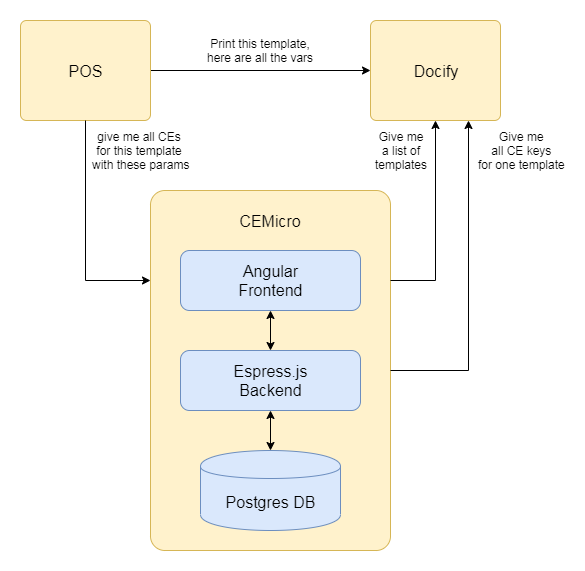
\includegraphics[width=0.6\linewidth]{assets/high-level-overview.png}
  \caption{High level context overview for the microservice}
  \label{fig:context}
\end{figure}

While the CEMicro service would become more complicated than at first anticipated, it was also decided to exclude some functionality from it. The reason is simply the limited time of the project, four months, and the nature of it being a proof of concept rather than a production-ready application.

One feature that was decided as out of scope for this project is user management or access control. The POS application has a relatively complex structure of access control with its various layers of authority, starting from the so-called HQ, the highest entity per market, through multiple levels of smaller and smaller organizational structures down to the local reseller. Each of these levels can define their own set of configuration options, which may or may not be overwritten by the next lower level of management. Because access control, especially such an elaborate one, adds another dimension of complexity to every project, it was decided to create this proof of concept without any, meaning there will only be one user who can do everything.

Another vital part of an application that was neglected is testing, both unit, and integration testing. Testing is more of an implementation detail and will, therefore, be further discussed in chapter \ref{sec:impl}.


\section{Understanding the existing feature}
\label{sec:arch:understanding}

\begin{itemize}
  \item \done{What is a configurable element?}
  \item \done{What properties does a CE have?}
  \item \done{Challenge: Understanding the task}
  \item \done{Challange/Example: Devs didn't know that CEs are not unique per template}
\end{itemize}

After defining what the microservice needs to accomplish and in what context it lives comes the next step in accurately understanding what functionality the new microservice needs to offer. Since we are extracting a microservice from an existing application, we are also extracting a specific feature set that users have been using and are used to.

Every application is faced with the question of how to expose data to the user and how to design a system's controls. In software development, this is usually called the user interface (UI) and user experience (UX). The ultimate goal is for the user interface to be intuitive to explain itself, but in any way, the user has to learn how to use the application. Even if the UI is terrible or even broken, the user will eventually learn how to use that system, even if he needs to use unintended detours to reach his goal. Once the user has determined the UI, every change will require him to re-learn even if the change is a fix of broken behavior.

An excellent example of this is Windows 8, where Microsoft decided to change the user interface of the start menu button. Every windows user has learned that the Windows Desktop is their default view, and the start menu serves as a hallway to all their applications and settings. As seen in figure \ref{fig:win8}, the start menu was removed in Windows 8 in favor of a hot corner that would lead to the new tiles interface. Even if the new interface would have been objectively better, with this decision, Microsoft asked every Windows user to re-learn one of the core concepts of its user interface. Not surprisingly, there was a huge outcry, and Microsoft quickly issued a patch with Windows 8.1 restoring the start menu the people were used to.

\begin{figure}
  \begin{subfigure}[b]{0.5\linewidth}
    
\includegraphics[width=\linewidth]{assets/windows-8-taskbar.png}
    \caption{Windows 8 taskbar without start menu button}
  \end{subfigure}
  \begin{subfigure}[b]{0.5\linewidth}
    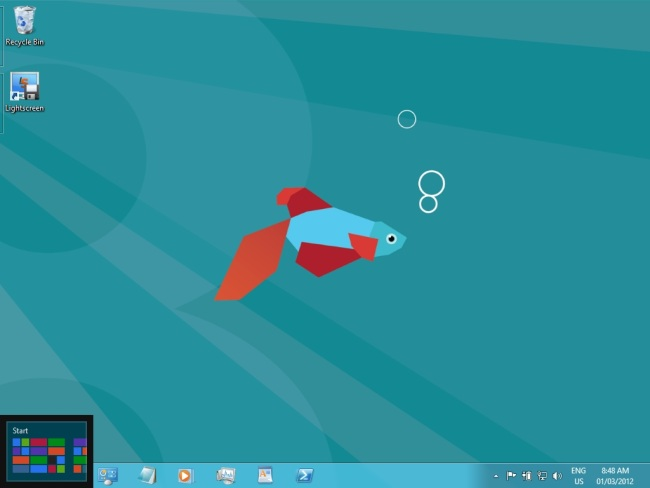
\includegraphics[width=\linewidth]{assets/windows-8-hot-corner.jpg}
    \caption{Windows 8 new hot corner}
  \end{subfigure}
  \caption{Windows 8 start menu UI change}
  \source{https://www.howtogeek.com/107662/how-to-live-without-the-start-button-in-windows-8/}
  \label{fig:win8}
\end{figure}

It is, therefore, imperative when extracting a microservice to understand precisely how the affected features were used by the existing users who will have to adapt to, or reject for that matter, the new service. Since I was not given a list of requirements or any sort of guideline about the precise workings of configurable elements, I took some time to understand the existing user interface and map out what kind of configurations are available to the user. The admin section for configurable element has three list view, figure \ref{fig:pos:a} shows the list of templates, figure \ref{fig:pos:c} the list of available CEs inside the selected template and figure \ref{fig:pos:b} shows a list of values that can be assigned to each CE grouped by hierarchy levels (Headquarter, MPC, etc.) and equipped witch a number of qualifying properties.

\begin{figure}
  \centering
  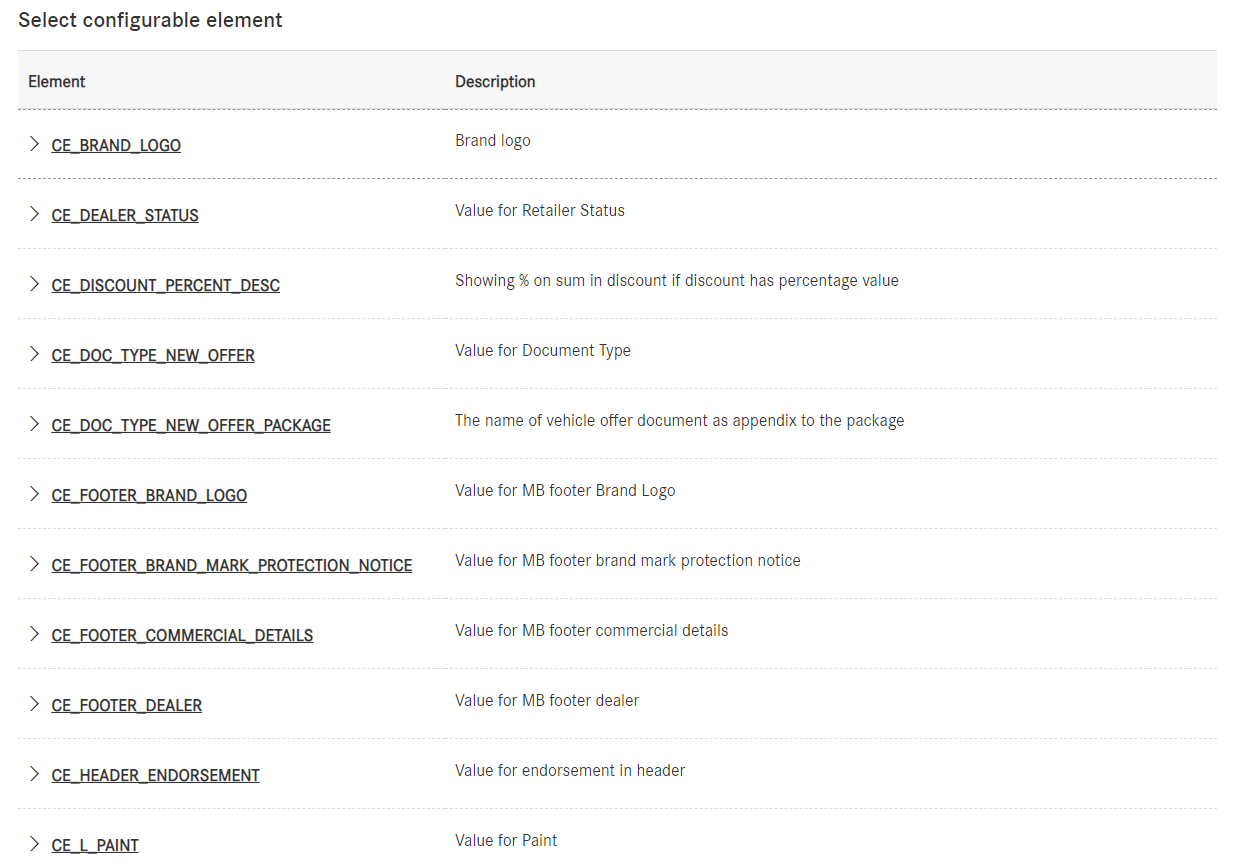
\includegraphics[width=0.75\linewidth]{assets/pos-ce-config-2.png}
  \caption{List of CE pertaining to a template}
  \label{fig:pos:c}
\end{figure}

This means CEs are not, as initially assumed, a simple key-value data structure but, in fact, can contain many values, each coming with a number of properties. These properties are later used to determine which value is the best fit for the current use case. Through testing, the possible values for each property were identified and mapped out in table \ref{table:ce-properties}. Figure \ref{fig:ce-properties} shows how these properties are presented to the user. Note how it is not immediately apparent that the valid from-to dates are part of the configuration and that they can, in fact, be changed. Also note the confusing layout of the value and description text inputs, the description which has no real purpose being the first input while the actual value of the configurable element, the most important thing of the whole interface, is the last input field of them all. Additionally, website users are more used to ``value'' fields being a single line and ``description'' fields being multi-line, here this logic is inverted.

\begin{table}[!ht]
  \begin{center}
    \begin{tabular}{|l|c|p{10cm}|}
      \hline
      Property & Required & Possible Values \\
      \hline\hline
      Name & * & [any] \\
      \hline
      Value & * & [any] \\
      \hline
      Description & & [any] \\
      \hline
      Language & & Any Language, English, German, French, ... \\
      \hline
      Paper Format & & Branded, Unbranded \\
      \hline
      Valid from-to & & [dates] \\
      \hline
      Vehicle type & & New Vehicle, Used Vehicle, Both \\
      \hline
      Division & & Any, MB Passenger Car, MB Van, Foreign Brand Passanger Car, MB Passenger Car \\
      \hline
      Brand & & Any, Mercedes Benz Passanger Cars, smart, Mercedes Benz, OTHER \\
      \hline
    \end{tabular}
  \end{center}
  \caption{Possible properties for configurable elements}
  \label{table:ce-properties}
\end{table}

\begin{figure}
  \centering
  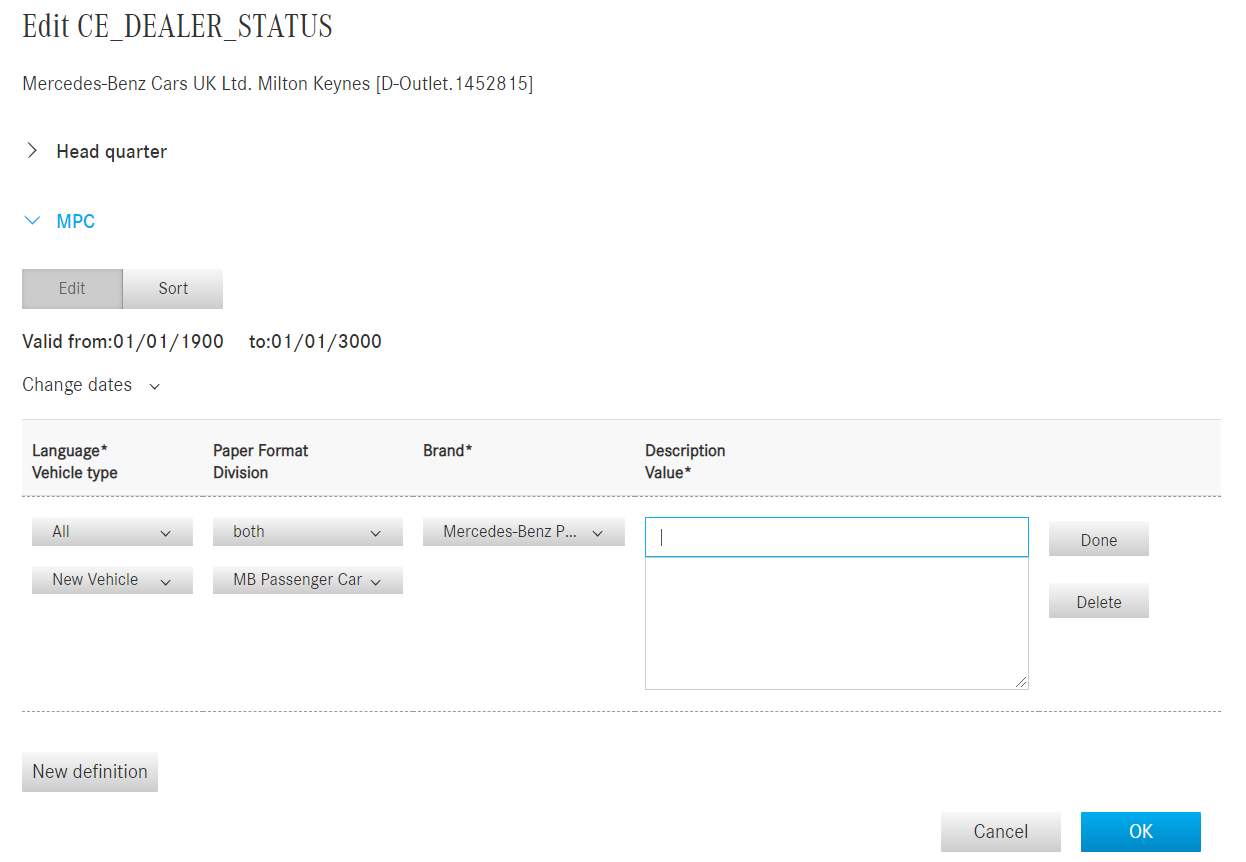
\includegraphics[width=0.8\linewidth]{assets/pos-ce-config-4.png}
  \caption{Configurable element configuration properties}
  \label{fig:ce-properties}
\end{figure}

The challenge of this task was, as already noted that no definite list of requirements or guidelines existed for the configurable elements feature, which should be extracted as a microservice. An intriguing detail showcasing this was my advisor's surprise when I told him that configurable element names are not treated as unique per templates, meaning if multiple templates contained CEs of the same name and the user would change the value of one, then the change was reflected for the other templates as well. I asked him if this was intended behavior, and he answered that he had always assumed the values to be unique to each template. I, therefore, decided to namespace the CEs with their respective market-templates tuple in the CEMicro application as this behavior was more intuitively expected.

Now that I had a comprehensive understanding of the current feature set for configurable elements, I could start drafting the user interface and application programming interface of the new CEMicro service.


\section{Deciding the Technology}
\label{sec:arch:technology}

I decided to build CEMicro as a modern web app. A web app is a website that behaves like an application instead of merely showing information to the user. It consists of three layers, as shown in the context diagram in figure \ref{fig:context}. The client is the user interface that the browser displays, the server provides the API and business logic for the client and the database to store the data.

The client is made up of a markup language HTML for the browser together with CSS for visual styling and a templating engine written in JavaScript, for which developers usually use a frontend framework. Javascript is a programming language that can run natively inside every browser. There are other languages a browser can run like Java, but only with appropriate plugins. While browser vendors first introduced JavaScript in the early days of the internet with the very first Netscape and Internet Explorer browsers, it has only become a viable choice for more ambitious projects during the last decade\footnote{I am writing this in 2020}. Only then the language became versatile enough and especially gained sufficient browser support to be considered for more significant projects. An excellent example of this is so-called promises, a data type needed for asynchronous programming, which both Chrome and Firefox only support since 2014 ~\cite{caniuse.2020} as seen on the graph in figure \ref{fig:caniuse-promises}.

\begin{figure}[ht]
  \centering
  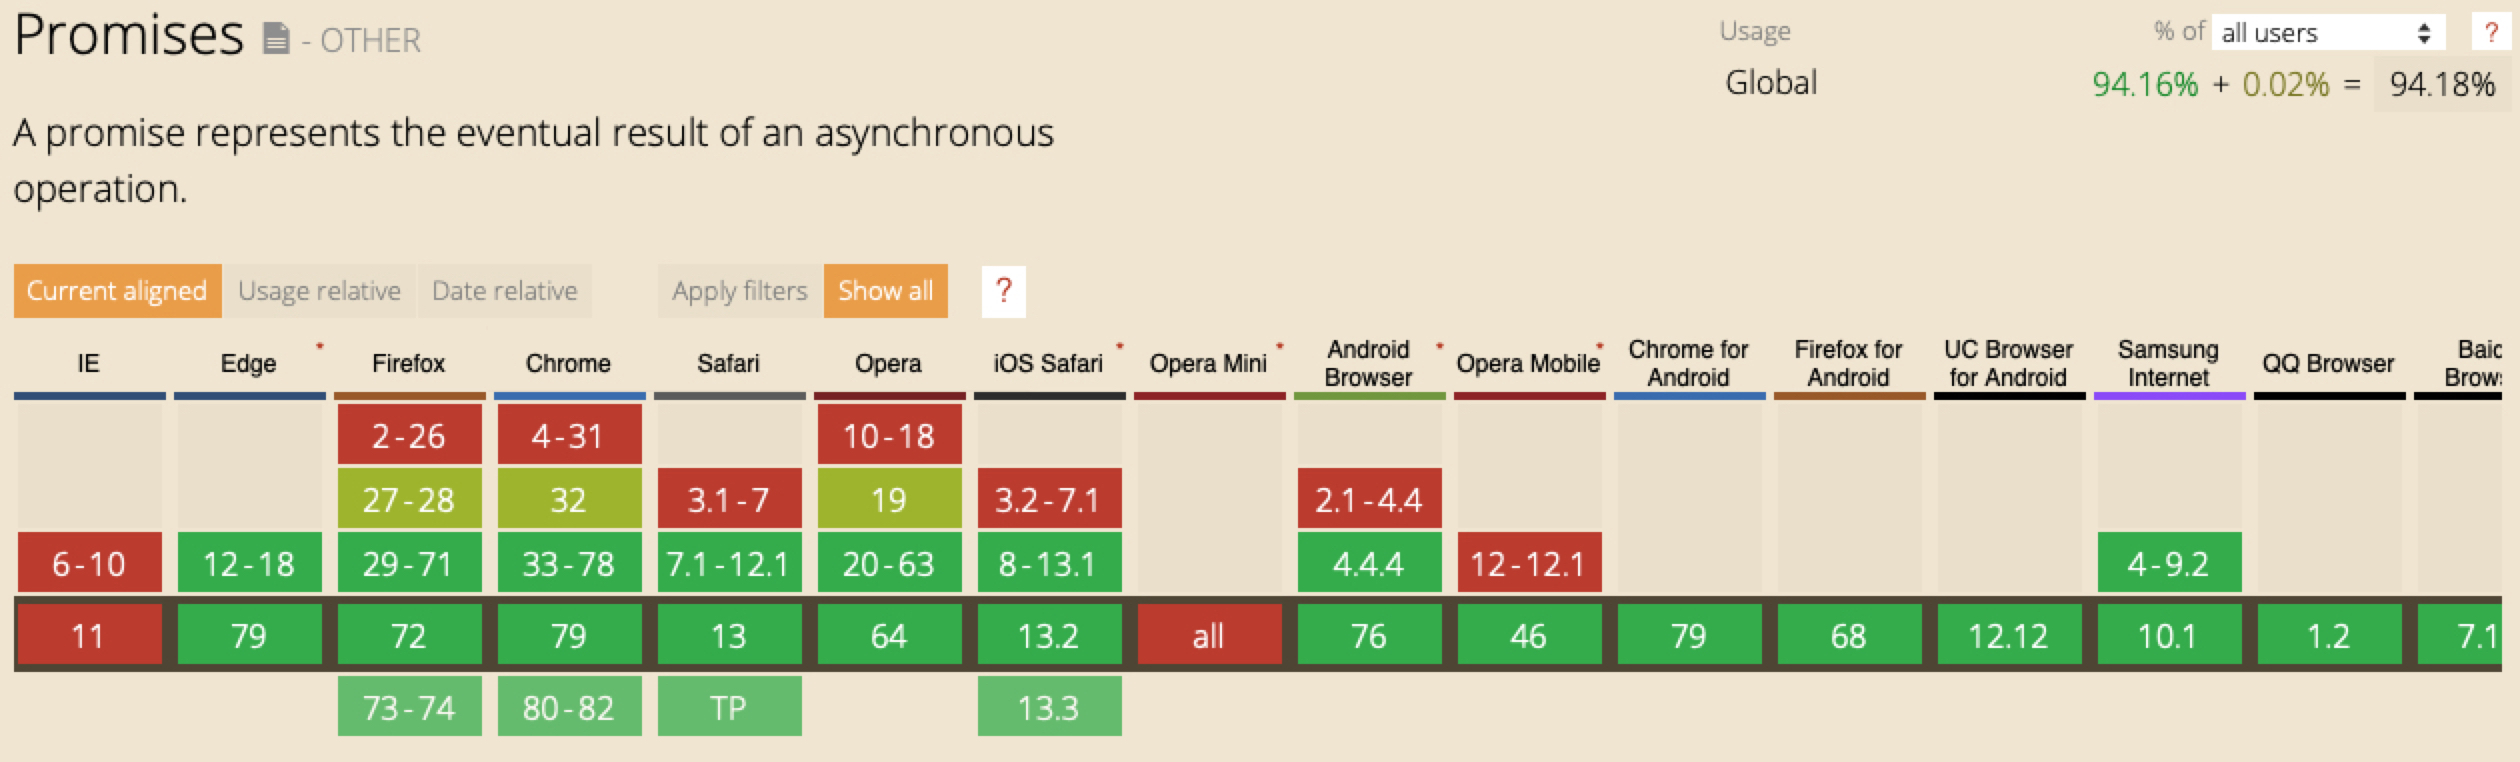
\includegraphics[width=0.8\linewidth]{assets/caniuse-promises.png}
  \caption{Browser support for JavaScript Promises}
  \source{https://caniuse.com/\#feat=promises}
  \label{fig:caniuse-promises}
\end{figure}

Developers often build a software project on top of a library or framework that handles all the infrastructure setup and allows the developers to focus on the main business logic. The POS application, for example, uses the Java Spring Framework. For the client-side of web apps, there are currently three big frameworks, namely React, Vue, and Angular, with React being the most popular, according to The State of Javascript Survey 2019, see figure \ref{fig:frontend-framework-usage} ~\cite{stateofjs.2019}. At first, I wanted to use Angular because the current Docify team who is also developing their application on a three-layer architecture with JavaScript for both client and server are using Angular as their client-side framework. However, after spending some time working with the framework, I decided to switch to Vue since Angular has a pretty steep learning curve, and I had already advanced experience with Vue from previous projects. Because the time for this thesis is limited to four months and the result is supposed to be a proof of concept, I felt justified in using a technology that I am more familiar with even though the local developer team at Capgemini is using a different framework.

\begin{figure}[ht]
  \centering
  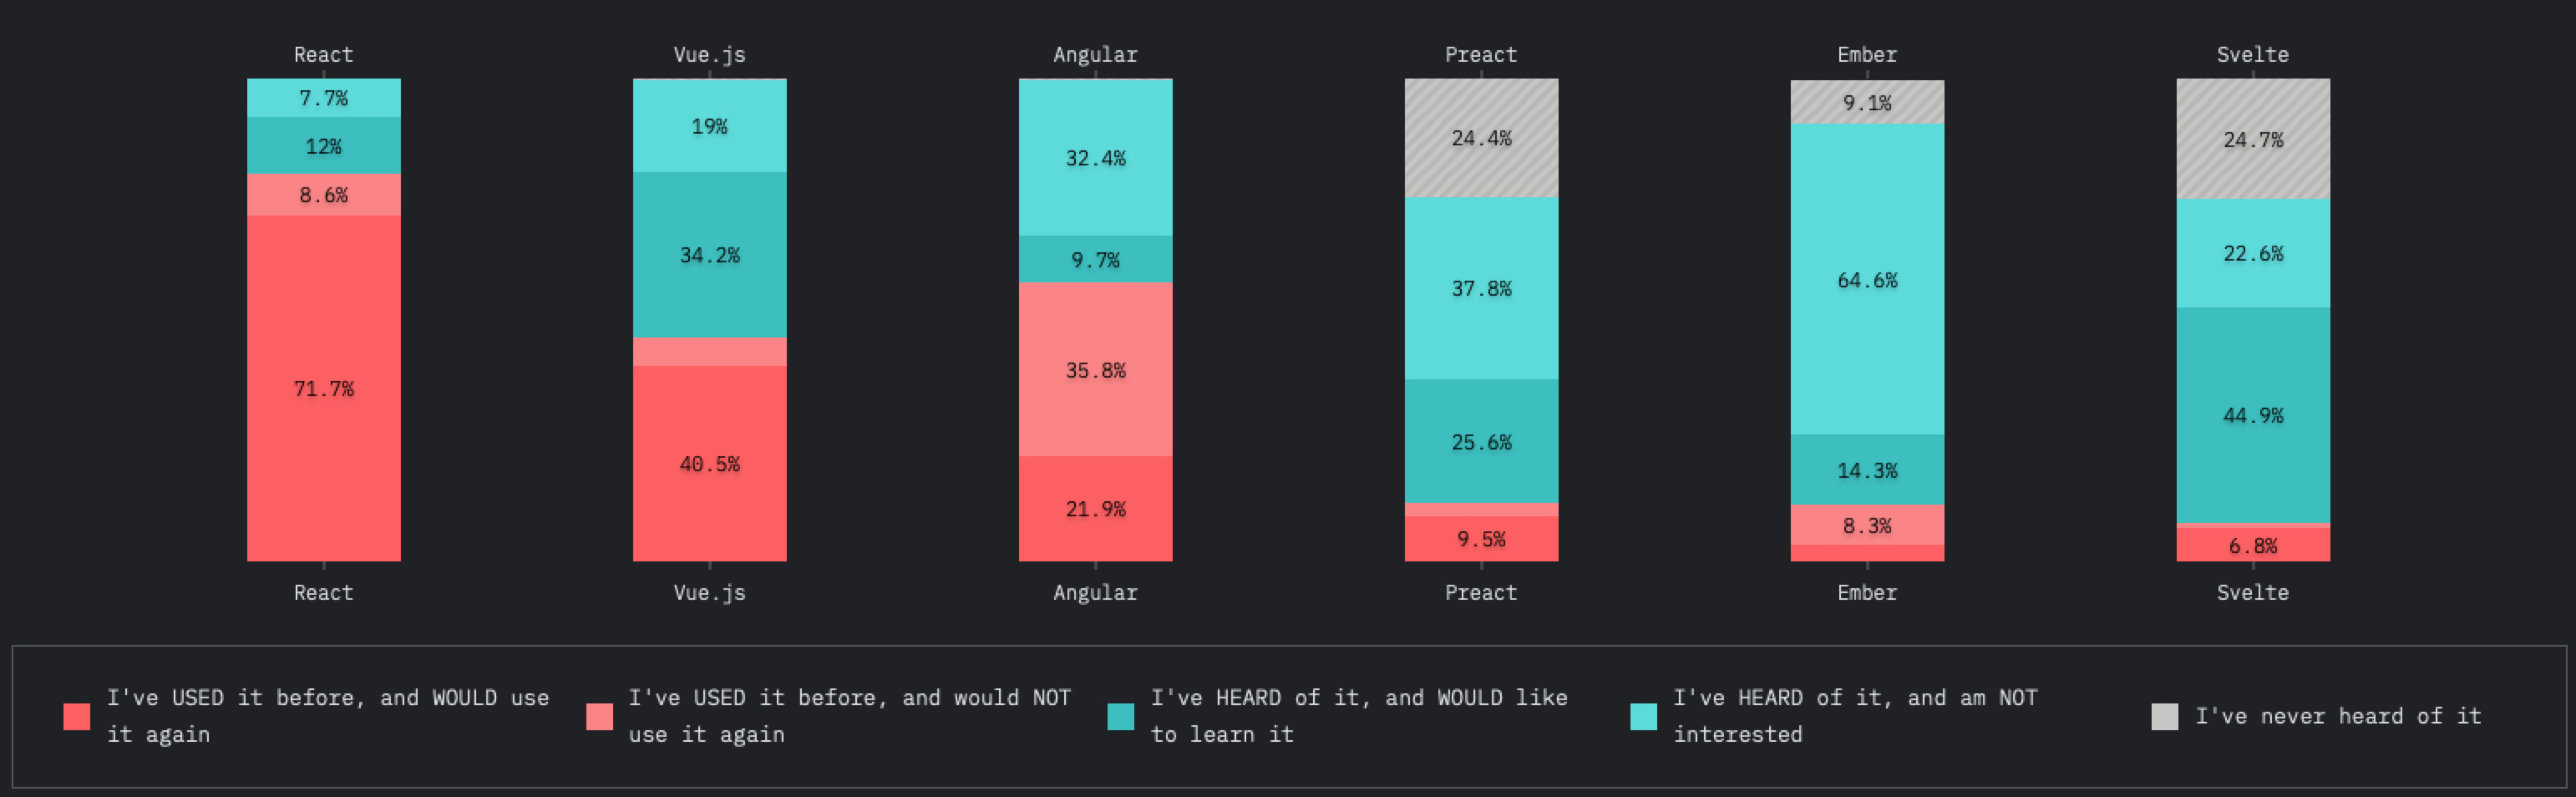
\includegraphics[width=0.8\linewidth]{assets/frontend-framework-usage.png}
  \caption{Usage statistics of current front end frameworks}
  \source{https://2019.stateofjs.com/front-end-frameworks/}
  \label{fig:frontend-framework-usage}
\end{figure}

Node.js is a runtime allowing the use of JavaScript on the server-side. Because the client-side of a web app has to use JavaScript, it is also an excellent choice for the server-side, thus the team only needs to have expertise in one programming language. The server-side framework the Docify team is using is called Express and is with 96\% awareness among JavaScript developers, basically the bread and butter tool for such a task ~\cite{stateofjs.2019}. The reason I am always referring to the Docify team is that, as already mentioned, they are the other microservice team using a JavaScript technology stack on the POS project. They are, therefore, my reference and, most likely, the people that continue the development of CEMicro after I finished.

PostgreSQL is the database that I am going to use for the data layer of CEMicro. It is the up and coming open-source relational database with a robust set of features ~\cite{stackoverflow.2019}. There are other databases out there like the more common MySQL and MongoDB, that uses an object-based system geared towards development with JavaScript. However, since once again, the Docify team is running PostgreSQL and the CEMicro service had no extraordinary requirements towards data persistence, I felt not much need to choose any other database system.

I want to mention one more technology outside the three-layer structure, which is vital to the idea of my task, and that is virtualization or containerization software. In the theoretical section about which problems microservices solve on page \pageref{sec:theory:what-problem}, one strong point in favor of this architecture model is the scalability argument. But for a service to be scalable, especially automatically in reaction to load, there needs to be a way to start and stop an instance of that service without manual interaction. Containerisation is not the first concept making this possible but by far the most sophisticated one. A container is an instance of a service that is self-contained, meaning it contains all the parts the software needs to run independently of the setup of the server. With the right software, such a container can then be started on any device and copied as often as needed. The right software for this is Docker, which has become the de-facto standard for containerization and is the most loved platform for this purpose among developers ~\cite{stackoverflow.2019}.

From the get-go, I developed CEMicro in a way that it can later run inside Docker containers. That means if you want to run CEMicro in the future, instead of needing to understand each technology and how to run it on your machine, all you need is one docker command, and the app is ready for use.


\section{Designing the User Interface}

\begin{itemize}
  \item \done{How can the complexity of CEs be exposed more straightforwardly?}
\end{itemize}

The user interface doesn't just serve an aesthetic purpose; it helps the user to understand and manage the complexity of a system. Figure \ref{fig:pos} on page \pageref{fig:pos} and figure \ref{fig:ce-properties} on page \pageref{fig:ce-properties} show glimpses of the existing user interface in POS. The existing interface is functional but clunky and hard to use. For example, it is not immediately apparent that the validity date of a CE can be changed and how to do it. It is also difficult to understand which of the CE items is active under which circumstances.

Figure \ref{fig:mockup} shows a high fidelity mockup I created before even starting to implement the microservice. I showed it to my mentor and the Docify team to get their feedback on the design. I tried to make the relationship between CEs and templates as simple as possible. Each CE can contain individual items, so I tried to show their hierarchy clearly. I also wanted to make all the different properties as evident as possible, showing them in a condensed view, highlighting the ones that differ from default values and only showing input options when the item is in edit mode.

\begin{figure}
  \centering
  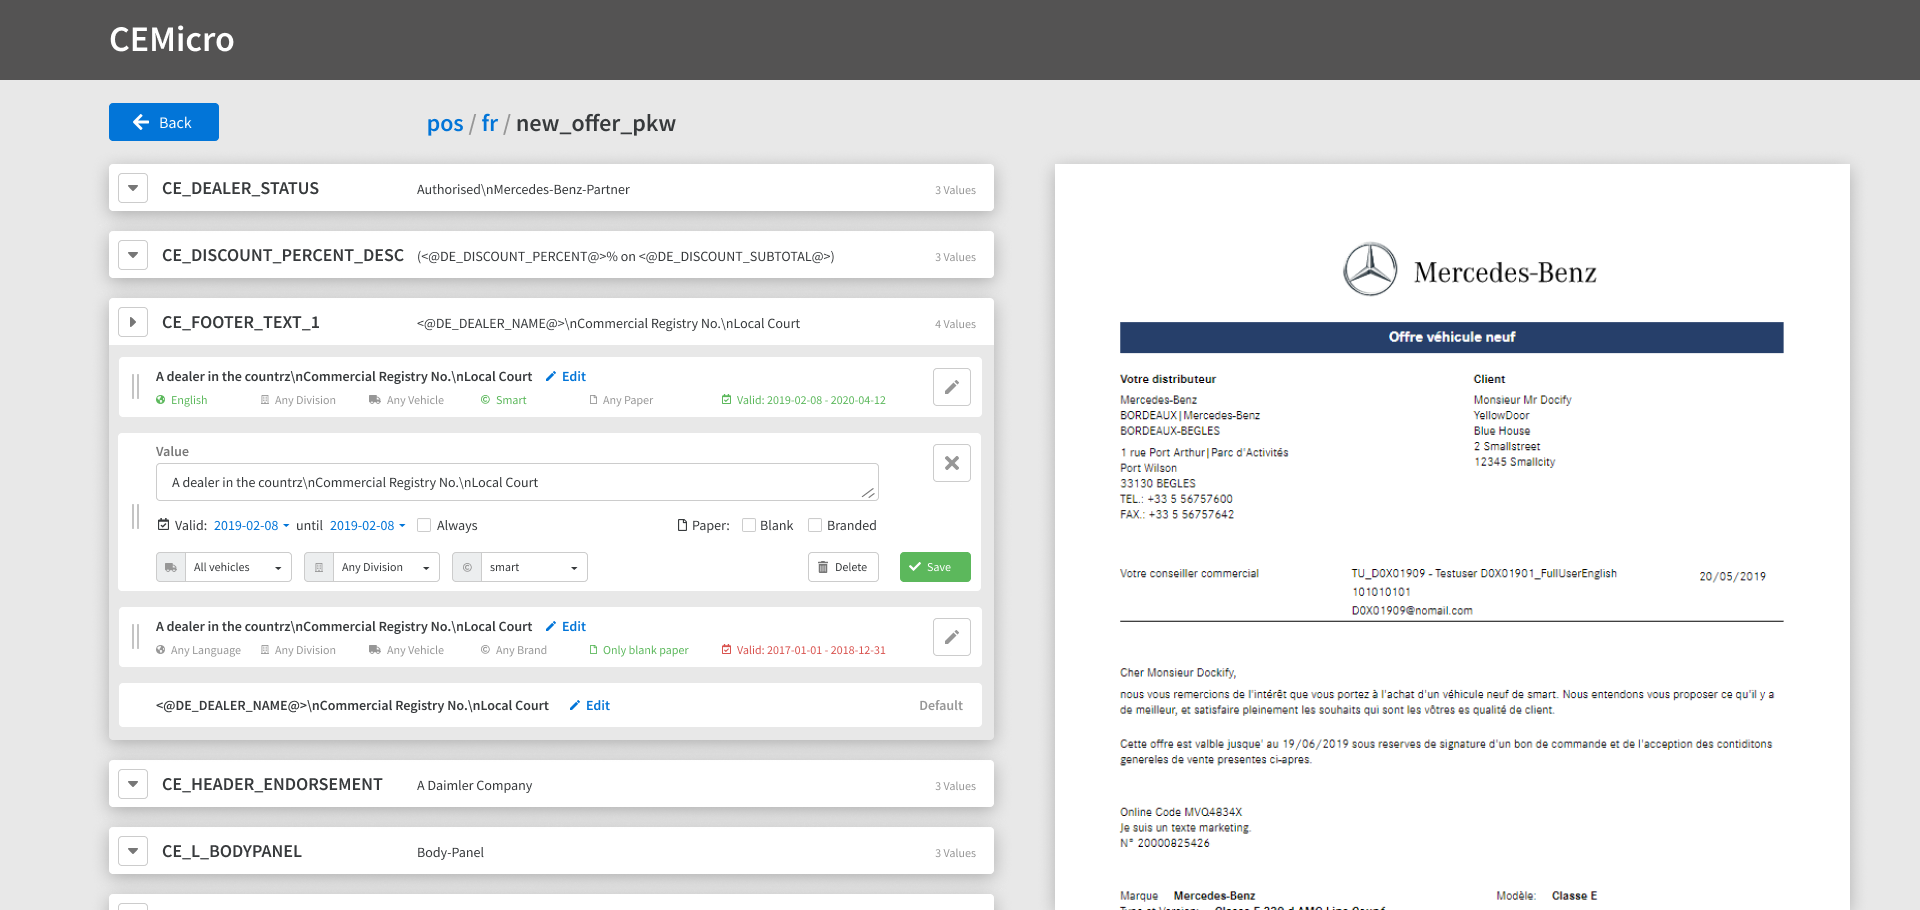
\includegraphics[width=\linewidth]{assets/cemicro-ui-mockup.png}
  \caption{User Interface mockup for CEMicro}
  \label{fig:mockup}
\end{figure}

In the final implementation, I decided to go with three views, always clearly showing the current position with breadcrumbs on top:

\begin{itemize}
  \item A list of templates (see figure \ref{fig:cemicro-template-list})
  \item A list of elements per template (see figure \ref{fig:cemicro-element-list})
  \item A list of items per element (see figure \ref{fig:cemicro-item-list})
\end{itemize}

The controls of a single element item became a little more uniform in the end. I also added a ``Refresh'' button above the document preview to see the current changes applied. I am planning another set of controls next to the refresh button to choose the properties (new vehicle vs. used vehicle, etc.), which should be applied to the preview to see which item is used under which circumstances. This last feature, however, is not yet implemented at the time of this writing.

\begin{figure}[ht]
  \begin{subfigure}[b]{0.5\linewidth}
    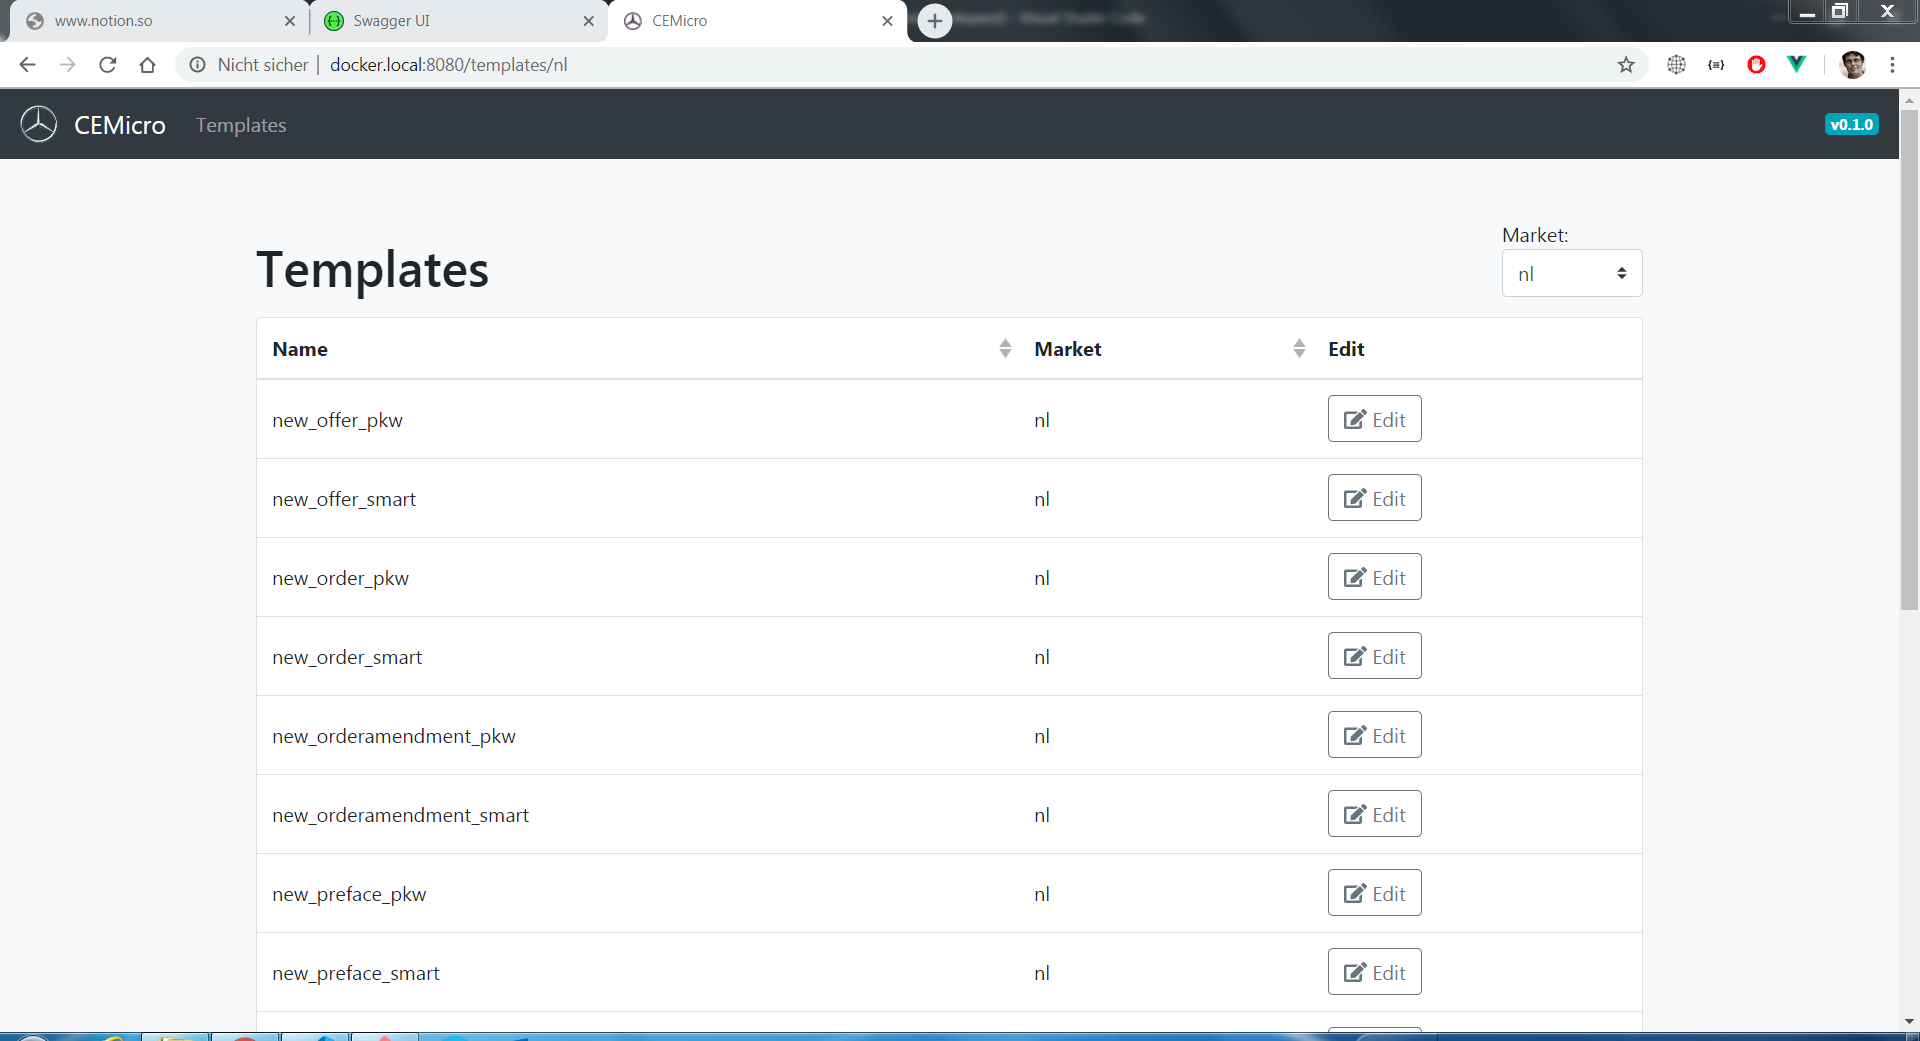
\includegraphics[width=\linewidth]{assets/cemicro-template-list.png}
    \caption{Template list view}
    \label{fig:cemicro-template-list}
  \end{subfigure}
  \begin{subfigure}[b]{0.5\linewidth}
    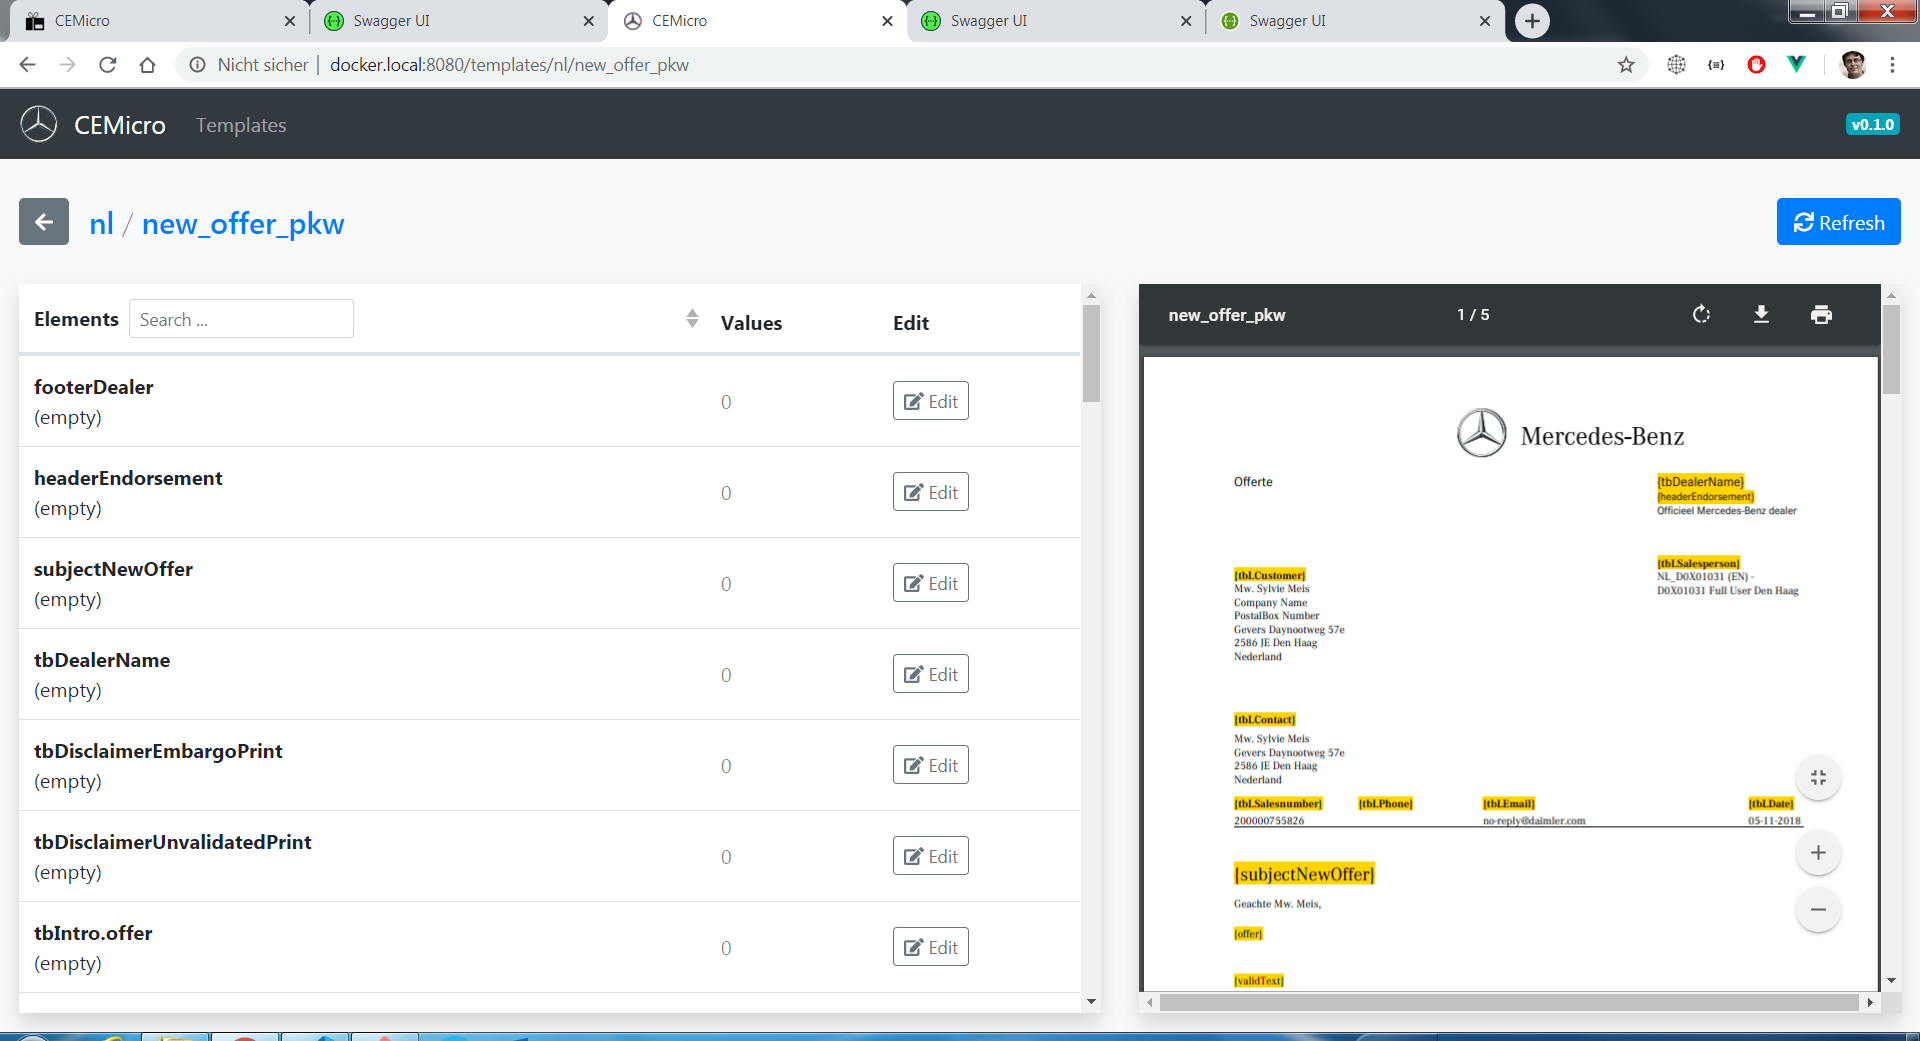
\includegraphics[width=\linewidth]{assets/cemicro-element-list.png}
    \caption{Configurable element view}
    \label{fig:cemicro-element-list}
  \end{subfigure}
  \begin{subfigure}[b]{0.5\linewidth}
    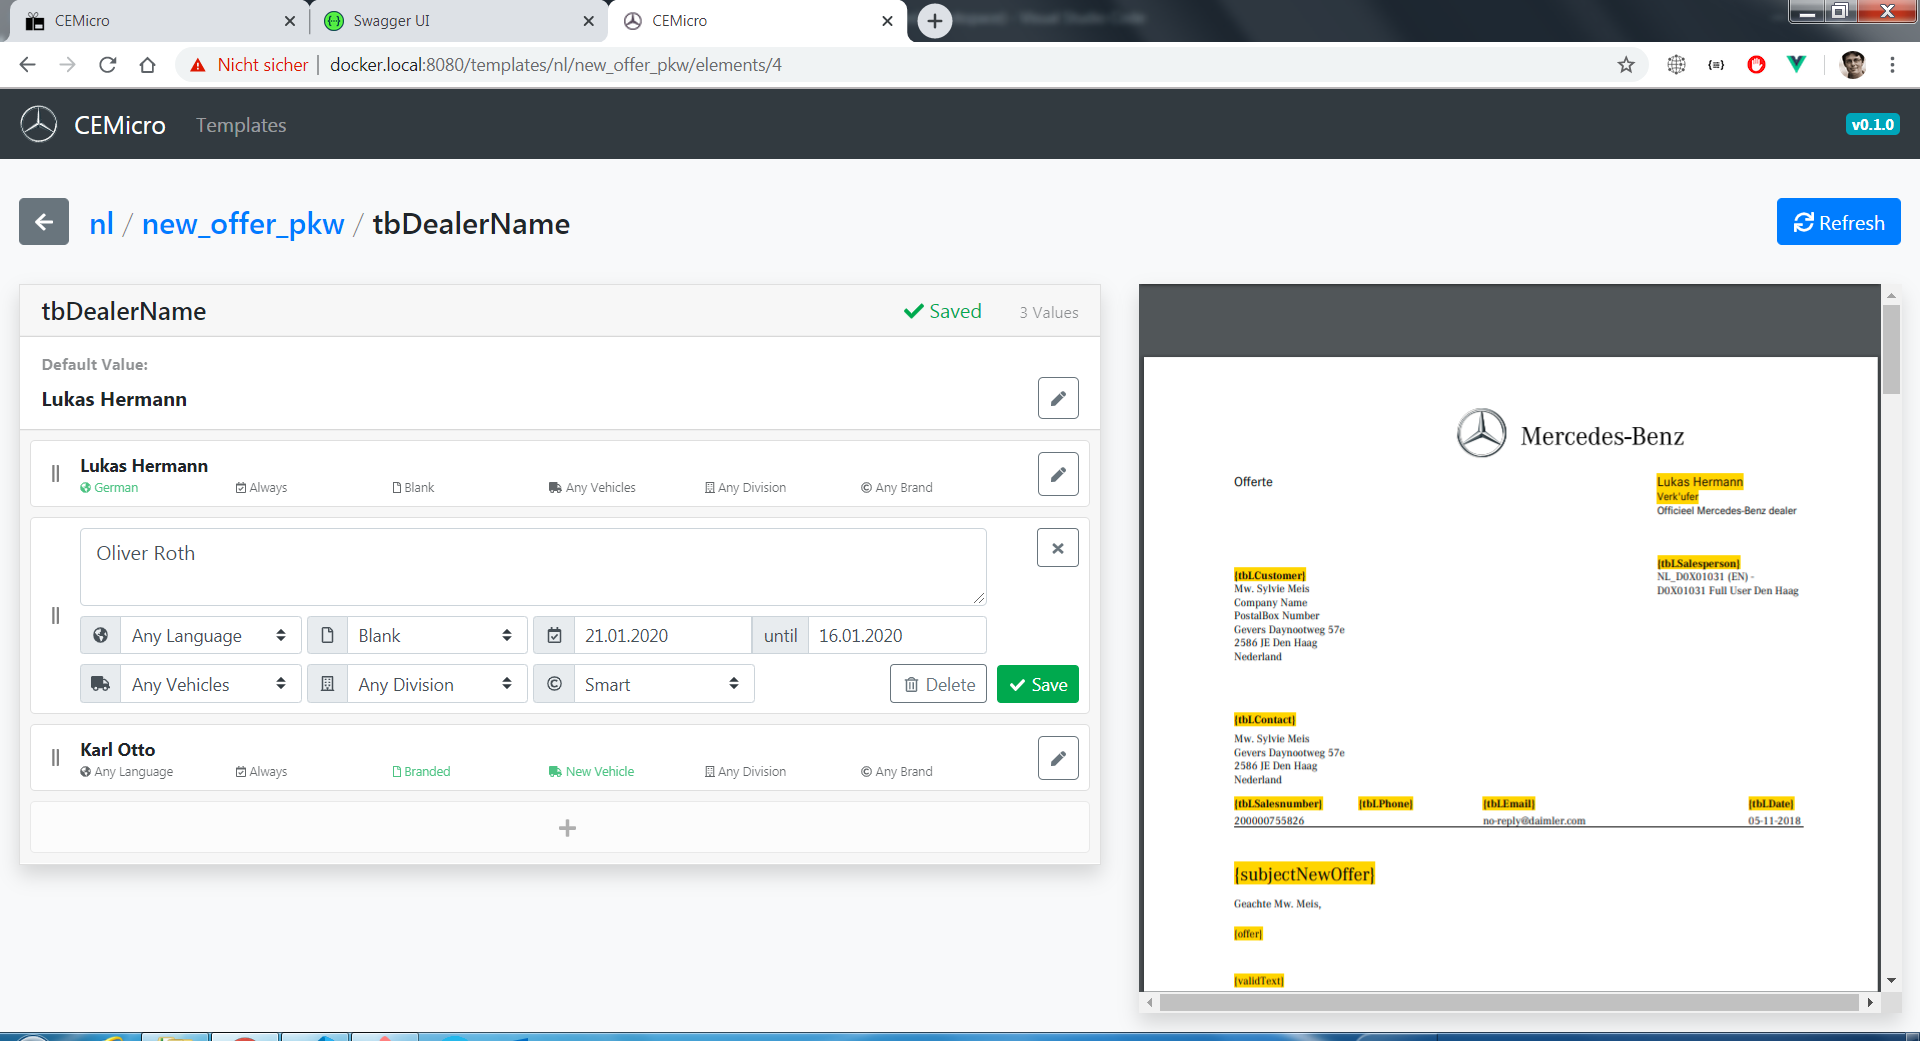
\includegraphics[width=\linewidth]{assets/cemicro-item-list.png}
    \caption{Element item view}
    \label{fig:cemicro-item-list}
  \end{subfigure}
  \caption{CEMicro user interface}
  \label{fig:cemicro-ui}
\end{figure}

\section{Wrap-up}

This part of the project, investigating the existing application, and making architectural decisions, provided the most learnings for me. The theory behind microservices was comparatively easy to understand because I worked a lot with cloud infrastructures before. The implementation was simple because I have ample experience in programming at this point. It was interesting how much complexity accrued over time in such a simple feature as the configurable elements. Deciding where the data should live helped me better understand how distributed data works. And redesigning an existing user interface is something I like doing.


